\documentclass[runningheads,a4paper]{llncs}
\usepackage{amssymb}
\setcounter{tocdepth}{3}
\usepackage{listings}
\usepackage{booktabs}
\usepackage{mathtools}
\usepackage{tabularx}
\usepackage{fixltx2e}
\usepackage[hyphens]{url}
\usepackage{hyperref}
\usepackage{upquote,textcomp}
\lstset{breaklines=true, basicstyle=\scriptsize\ttfamily, upquote=true}

\usepackage{fancyvrb}
\VerbatimFootnotes
\usepackage{cprotect}

\usepackage{graphicx}
\makeatletter
\def\maxwidth#1{\ifdim\Gin@nat@width>#1 #1\else\Gin@nat@width\fi}
\makeatother

\usepackage{amsmath}
\usepackage{color,graphics,array,csscolor}
\usepackage{pmml-new}

\usepackage{fontspec,unicode-math}
\usepackage[Latin,Greek]{ucharclasses}
\setTransitionsForGreek{\fontspec{Times New Roman}}{}

\usepackage{subscript}
\lstset{breaklines=true, basicstyle=\scriptsize\ttfamily}

\usepackage[margin=1.89in]{geometry}

\begin{document}
\mainmatter

\title{Freedom for bibliographic references:\\ OpenCitations arise}
\titlerunning{Freedom for bibliographic references}
\author{Silvio Peroni\inst{1} \and
David Shotton\inst{2} \and
Fabio Vitali\inst{1}}
\authorrunning{Silvio Peroni et al.}
\institute{DASPLab, DISI, University of Bologna, Bologna, Italy\and
Oxford e-Research Centre, University of Oxford, Oxford, UK\\
\email{silvio.peroni@unibo.it, 
david.shotton@oerc.ox.ac.uk, 
fabio.vitali@unibo.it}}
\maketitle

\begin{abstract}
Scholarly citations from one publication to another, expressed as reference lists within academic articles, are core elements of scholarly communication. Unfortunately, they usually can be accessed {\em en masse }only by paying significant subscription fees to commercial organizations, while those few services that do made them available for free impose strict limitations on their reuse. In this paper we provide an overview of the OpenCitations Project (\url{http://opencitations.net}) undertaken to remedy this situation, and of its main product, the OpenCitations Corpus, which is an open repository of accurate bibliographic citation data harvested from the scholarly literature, made available in RDF under a Creative Commons public domain dedication.

{\bf RASH version:} \url{https://w3id.org/oc/paper/occ-lisc2016.html}

\keywords{Citation Database, OpenCitations, OpenCitations Corpus, Scholarly Communication, Semantic Publishing}
\end{abstract}


\section{Introduction}

Databases of citation data are among the most attractive and used artefacts in the Scholarly Communication domain. They are one of the main tools used by researchers for gaining knowledge about a particular topic, and by scientists in Bibliometrics, Informetrics, and Scientometrics for analysing the complex relationships that exist within huge networks of citations of scholarly works. They also serve institutional goals, since they provide one of the main mechanisms for assessing the quality of research by means of (sometimes questionable) metrics and indicators calculated from such citation databases. While some of these resources, e.g. Microsoft Academic Graph\footnote{\url{https://www.microsoft.com/en-us/research/project/microsoft-academic-graph/}} and Google Scholar\footnote{\url{https://scholar.google.com/}}, are freely accessible (but not downloadable), those considered the most authoritative by institutions worldwide, namely Scopus\footnote{\url{https://www.scopus.com/}} and Web of Science\footnote{\url{http://webofscience.com/}}, can be accessed only by paying significant access fees, which may amount to tens of thousands of pounds annually  \cite{__RefNumPara__293_1852566440}.

Reference lists within academic articles are core elements of scholarly communication, since they both permit the attribution of credit and integrate our independent research endeavours. But the cruel reality is that these key data are not freely available. In the current age where Open Access is considered a necessary practice in research, it is a scandal that reference lists from scholarly publications (conference papers, books, journal articles, etc.) are not readily and freely available for use by all scholars. As we have already stated in a previous work  \cite{__RefNumPara__293_1852566440}: 

\begin{quote}
Citation data now needs to be recognized as a part of the Commons -- those works that are freely and legally available for sharing -- and placed in an open repository, where they should be stored in appropriate machine-readable formats so as to be easily reused by machines to assist people in producing novel services.
\end{quote}

This is the main premise behind the OpenCitations Project  \cite{__RefNumPara__293_1852566440} \cite{__RefNumPara__6041_1890349413}, which has created an open repository of scholarly citation data -- the OpenCitations Corpus (OCC) -- made available under a Creative Commons public domain dedication\footnote{\url{https://creativecommons.org/publicdomain/zero/1.0/legalcode}} to provide in RDF accurate citation information (bibliographic references) harvested from the scholarly literature. Since the beginning of July 2016, the OCC has been ingesting and processing the reference lists of scholarly papers available in Europe PubMed Central\footnote{\url{http://europepmc.org/}}. In this paper we provide a brief overview of the OCC's main components that make possible the extraction, a description of such reference lists in RDF, and a progress report concerning the available citation data.

The rest of the paper is organised as follows. In Section~\ref{__RefHeading__5190_1890349413} we recall the story of the OpenCitations Project since its beginning in 2010. In Section~\ref{__RefHeading__151_1852566440} we describe the revised metadata specification and software tools that have been recently developed within the OpenCitations Project for the creation of a new and improved instantiation of the OCC. In Section~\ref{__RefHeading__5192_1890349413} we briefly describe other open (and RDF-based) repositories of scholarly document metadata. Finally, in Section~\ref{__RefHeading__171_1852566440}, we sketch out our future plans.

\section{The story so far}\label{__RefHeading__5190_1890349413}

The OpenCitations Project formally started in 2010 as a one-year project funded by JISC\footnote{\url{http://www.jisc.ac.uk/whatwedo/programmes/inf11/jiscexpo/jiscopencitation.aspx}} (subsequently extended for an additional half year), with David Shotton as director, who at that time was working in the Department of Zoology at the University of Oxford. The project's goal was global in scope, and was designed to change the face of scientific publishing and scholarly communication, since it aimed to publish bibliographic citation information in RDF and to make citation links as easy to traverse as Web links. The main deliverable of the project, among several outcomes\footnote{\url{https://opencitations.wordpress.com/2011/07/01/jisc-open-citations-project-–-final-project-blog-post/}}, was the release of an open repository of scholarly citation data described using the SPAR (Semantic Publishing and Referencing) Ontologies\footnote{\url{http://www.sparontologies.net/}} \cite{__RefNumPara__17_1852566440}, namely the OpenCitations Corpus, initially populated with the citations from journal articles within the Open Access Subset of PubMed Central\footnote{\url{http://www.ncbi.nlm.nih.gov/pmc/tools/openftlist/}} \cite{__RefNumPara__6041_1890349413}.

In May 2014, OpenCitations was adopted by the Infrastructure Services for Open Access (IS4OA)\footnote{\url{https://is4oa.org/services/open-citations-corpus/}} as one of its academic Open Access services. IS4OA is UK-based not-for-profit charitable company that aims to provide benefit to the global community of research information users. It acts as an umbrella organisation that supports openly accessible information and discovery services relating to academic information, research results and scholarly publications, by providing business structure and expertise and a means of channelling financial support to these services.

At the end of 2015, Silvio Peroni joined the OpenCitations Project as co-director, with the aim of setting up a new instantiation of the Corpus based on a new metadata schema and employing several new technologies to automate the ingestion of fresh citation metadata from authoritative sources. The current instantiation of the OCC is hosted by the Department of Computer Science and Engineering (DISI) at the University of Bologna, and since the beginning of July 2016 it has been ingesting, processing and publishing reference lists of scholarly papers available in Europe PubMed Central, as described in the following section.

\section{The new instantiation of the OpenCitations Corpus}\label{__RefHeading__151_1852566440}

The OpenCitations Project (\url{http://opencitations.net}) has recently created a new instantiation of its open citations database, with an integrated SPARQL endpoint and a browsing interface to support data consumers. This database, the OpenCitations Corpus (OCC), is an open repository of scholarly citation data made available under a Creative Commons public domain dedication (CC0), which provides accurate bibliographic references harvested from the scholarly literature, described using the SPAR Ontologies  \cite{__RefNumPara__17_1852566440} according to the OCC metadata document  \cite{__RefNumPara__19_1852566440}, that others may freely build upon, enhance and reuse for any purpose, without restriction under copyright or database law.

\subsection{The model}\label{__RefHeading__5535_1890349413}

The newly revised metadata model used for the data stored in the OCC, available at  \cite{__RefNumPara__19_1852566440} and briefly summarised in Fig.~\ref{refIllustration2}, is explicitly aligned with the SPAR Ontologies  \cite{__RefNumPara__17_1852566440} and other standard vocabularies. In particular:
\begin{itemize}
\item the FRBR-aligned Bibliographic Ontology (FaBiO)\footnote{\url{http://purl.org/spar/fabio}} \cite{__RefNumPara__7775_1890349413} is used to provide a description of all the metadata of citing/cited bibliographic resources (conference papers, book chapters, journal articles, etc.) and their related container resources (academic proceedings, books, journals, etc.), and metadata about the particular formats in which they have been embodied (digital vs. print, first and ending pages, etc.);
\item the Publishing Roles Ontology (PRO)\footnote{\url{http://purl.org/spar/pro}} \cite{__RefNumPara__7993_1890349413} is used to describe the roles of bibliographic agents (author, editor, publisher, etc.) related to the bibliographic resources, while the order among such roles, e.g. the list of authors of a paper, is handled by extending PRO with an additional property, i.e. \Verb+oco:hasNext+;
\item the Bibliographic Reference Ontology (BiRO)\footnote{\url{http://purl.org/spar/biro}} and the Citation Counting and Context Characterization Ontology (C4O)\footnote{\url{http://purl.org/spar/c4o}} \cite{__RefNumPara__8388_1890349413} are used to describe the textual content of each reference in the reference list of a citing bibliographic resource;
\item finally, the DataCite Ontology\footnote{\url{http://purl.org/spar/datacite}} is used to define all the identifiers (e.g. DOI, PubMed ID, PubMed Central ID, ORCID, ISSN, etc.) for bibliographic resources and the agents involved, while the Friend Of A Friend (FOAF)\footnote{\url{http://xmlns.com/foaf/spec/}} ontology is used to define additional data about agents, such as their given and family names.
\end{itemize}

For convenience, all the terms from the aforementioned ontologies are collected within a new ontology called the OpenCitations Ontology (OCO)\footnote{\url{https://w3id.org/oc/ontology}}. This is not yet another bibliographic ontology, but rather just a mechanism for grouping existing complementary ontological entities from several other ontologies for the purpose of providing descriptive metadata for the OCC.
\begin{figure}[h!]
\centering
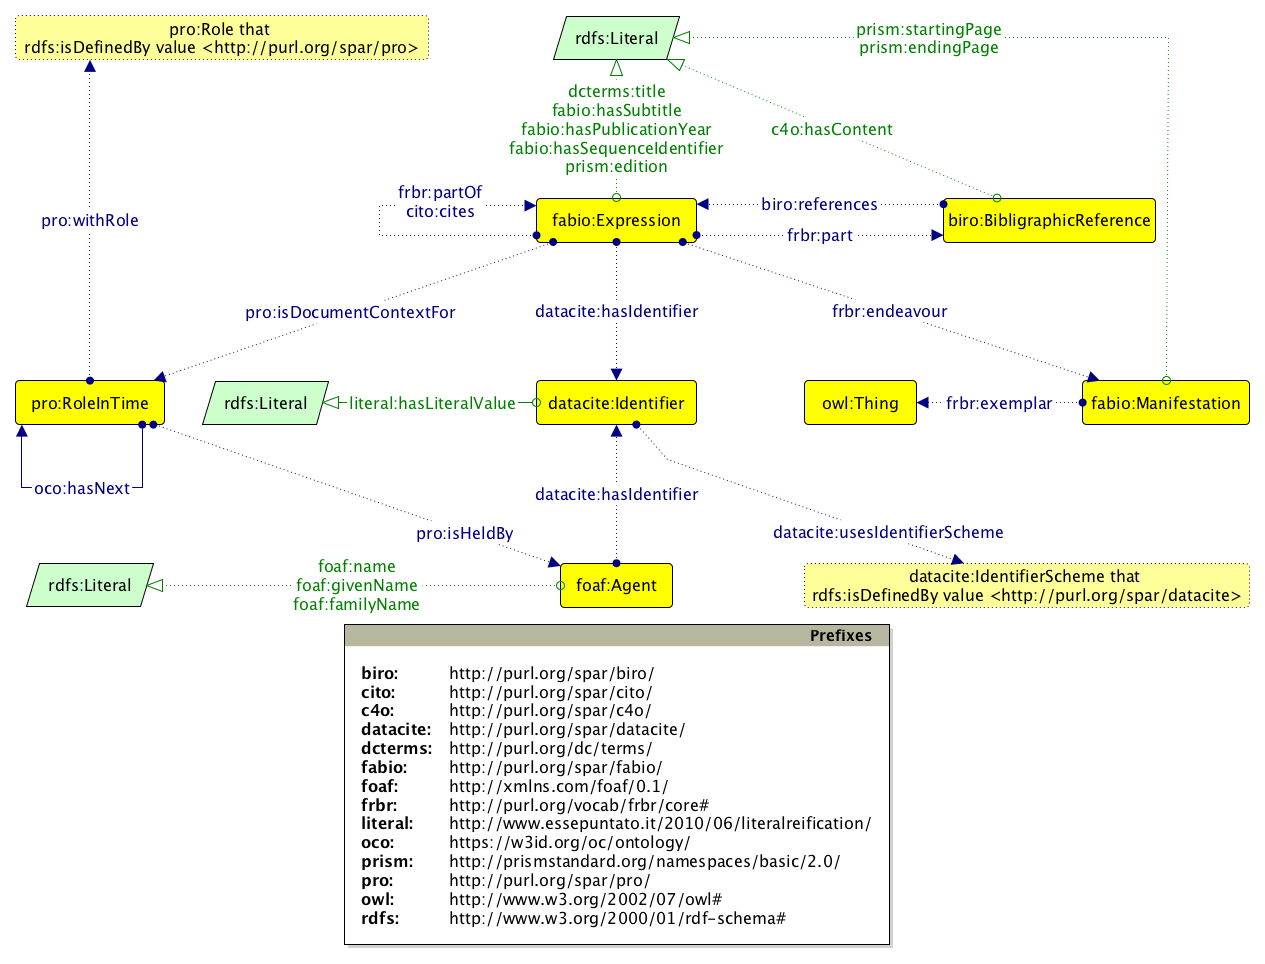
\includegraphics[width=\maxwidth{\textwidth}]{img/10000000000004F1000003C40B1D2514.png}
\cprotect\caption{The Graffoo diagram  \cite{__RefNumPara__6706_524287244} of the main ontological entities described by the OCC metadata model.}
\label{refIllustration2}
\end{figure}


\subsection{The data}\label{__RefHeading__10638_1890349413}

The OCC stores metadata relevant to bibliographic citations in RDF, encoded as JSON-LD\footnote{\url{http://json-ld.org/}}. In early September 2016, all the ingested data will be also available as downloadable datasets. In the meantime, two exemplar dataset, compliant with the OCC metadata model introduced in Section~\ref{__RefHeading__5535_1890349413}, have been made available: the first from article metadata provided by Springer Nature (available at  \cite{__RefNumPara__5447_1890349413}), and the second gathered from Europe PubMed Central (available at  \cite{__RefNumPara__5449_1890349413})\footnote{All the resources in the exemplar datasets have URLs that starts with ``\url{http://localhost:8000/corpus/}'' and do not refer to any existing IRI included in the current version of the corpus.}. 

The following six bibliographic entity types occur in the OCC, as well as in the aforementioned exemplar datasets:
\begin{itemize}
\item {\bf bibliographic resources} (br), class \Verb+fabio:Expression+ -- resources that either cite or are cited by other bibliographic resources (e.g. journal articles), or that contain such citing/cited resources (e.g. journals);
\item {\bf resource embodiments} (re), class \Verb+fabio:Manifestation+ -- details of the physical or digital forms in which the bibliographic resources are made available by their publishers;
\item {\bf bibliographic entries} (be), class \Verb+biro:BibliographicReference+ -- the literal textual bibliographic entries occurring in the reference lists within the bibliographic resources, that reference other bibliographic resources;
\item {\bf responsible agents} (ra), class \Verb+foaf:Agent+ -- names of agents having certain roles with respect to the bibliographic resources (i.e. names of authors, editors, publishers, etc.);
\item {\bf agent roles} (ar), class \Verb+pro:RoleInTime+ -- roles held by agents with respect to the bibliographic resources (e.g. author, editor, publisher);
\item {\bf identifiers} (id) (class \Verb+datacite:Identifier+) -- external identifiers (e.g. DOI, ORCID, PubMedID) associated with the bibliographic entities.
\end{itemize}

The corpus URL (\url{https://w3id.org/oc/corpus/}) identifies the entire OCC, which is composed of several sub-datasets, one for each of the six aforementioned bibliographic entities included in the corpus. Each of these has a URL composed by suffixing the corpus URL with the two-letter short name for the class of entity (e.g. ``be'' for a bibliographic entry) followed by an oblique slash (e.g. \url{https://w3id.org/oc/corpus/be/}). Each dataset is described appropriately by means of the Data Catalog Vocabulary\footnote{\url{https://www.w3.org/TR/vocab-dcat/}} and the VoID Vocabulary\footnote{\url{https://www.w3.org/TR/void/}}, and a SPARQL endpoint\footnote{\url{http://w3id.org/oc/sparql}} is made available for all the entities included in the entire OCC.

Upon initial curation into the OCC, a URL is assigned to each entity within each sub-dataset, which can be accessed in different formats (HTML, RDF/XML, Turtle, and JSON-LD) via content negotiation. Each entity URL is composed by suffixing the sub-dataset URL with a number assigned to each resource, unique among resources of the same type, which increments for each new entry added to that resource class. For instance, the resource \url{https://w3id.org/oc/corpus/be/537} is the 537\textsuperscript{th} bibliographic entry recorded within the OCC. The final part of such URL, i.e. the two-letter short name for the class of items plus ``/'' plus the number (``be/537'' in the example), is called the internal {\em corpus identifier}, since it allows the unique identification of any entity within the OCC.

Each of these entities has associated metadata describing its provenance using the PROV-O\footnote{\url{https://www.w3.org/TR/prov-o/}} ontology and its PROV-DC extension\footnote{\url{https://www.w3.org/TR/prov-dc/}} (e.g. \url{https://w3id.org/oc/corpus/be/537/prov/se/1}). In particular, we keep track of the curatorial activities related to each OCC entity, the curatorial agents involved, and their roles. 

All these RDF data are stored in BibJSON\footnote{\url{http://okfnlabs.org/bibjson/}} encoded as JSON-LD, defined through an appropriate JSON-LD context\footnote{\url{https://w3id.org/oc/corpus/context.json}} which hides the complexity of the model (shown in Fig.~\ref{refIllustration2}) behind natural language keywords. For instance, the following excerpt is the JSON-LD linearisation of the aforementioned ``be/537'' entity:

\begin{lstlisting}[mathescape]
{
  "iri": "gbe:537", 
  "a": "entry", 
  "label": "bibliographic entry 537 [be/537]", 
  "content": "Svahn, HA, Berg, A. Single cells or large populations, Lab Chip, 2007, 7, 544, 546, DOI: 10.1039/b704632b, PMID: 17476370", 
  "crossref": "gbr:1601"
}
\end{lstlisting}

In this excerpt, ``iri'' defines the URL of the resource in consideration (where ``gbe:'' is a prefix for ``https://w3id.org/oc/corpus/be/''), while ``a'', ``entry'', ``label'', ``content'' and ``crossref'' stand for \Verb+rdf:type+, \Verb+biro:Biblio+ \Verb+graphicReference+, \Verb+rdfs:label+, \Verb+c4o:hasContent+ and \Verb+biro:references+ respectively (where ``gbr:'' is a prefix for ``https://w3id.org/oc/corpus/br/'').

Additional information about OCC's handling of citation data, and the way they are represented in RDF, are detailed in the official OCC Metadata Document  \cite{__RefNumPara__19_1852566440}.

\subsection{The ingestion workflow}

The ingestion of citation data into the OCC is handled by two Python scripts called {\em Bibliographic Entries Extractor} ({\em BEE}) and the {\em SPAR Citation Indexer} ({\em SPACIN}), available in the OCC's GitHub software repository\footnote{\url{https://github.com/essepuntato/opencitations}}.

\subsubsection{BEE -- The Bibliographic Entries Extractor}\label{__RefHeading__11281_1890349413}

As shown Fig.~\ref{refIllustration0}, BEE is responsible for the creation of JSON files containing information about the articles in the OA subset of PubMed Central (retrieved by using the Europe PubMed Central API\footnote{\url{https://europepmc.org/RestfulWebService}}). Each of these JSON files is created by asking Europe PubMed Central about all the metadata of the articles it stores that have available the source XML file. Once identified, BEE processes all the XML sources so as to extract the complete reference list of each paper under consideration, and includes all the data in the final JSON file. An excerpt of one of those JSON files is as follows:

\begin{lstlisting}[mathescape]
{
  "doi": "10.1007/s10544-016-0081-z", 
  "pmid": "27299468", 
  "pmcid": "PMC4908161",
  "localid": "MED-27299468", 
  "curator": "BEE EuropeanPubMedCentralProcessor", 
  "source": "http://www.ebi.ac.uk/europepmc/webservices/rest/PMC4908161/fullTextXML", 
  "source_provider": "Europe PubMed Central", 
  "references": [
    ... 
    {
      "bibentry": "Svahn, HA, Berg, A. Single cells or large populations, Lab Chip, 2007, 7, 544, 546, DOI: 10.1039/b704632b, PMID: 17476370", 
      "pmid": "17476370", 
      "doi": "10.1039/b704632b", 
      "process_entry": "True"
    },
    ...
  ] 
}
\end{lstlisting}

In particular, for each articles retrieved by means of the Europe PubMed Central API, BEE stores all the available bibliographic identifiers (in the example, ``doi'', ``pmid'', ``pmcid'', and ``localid'') and all the textual references, enriched by their own related bibliographic identifiers if those are available. In addition, the JSON file also includes provenance information about the source, its provider and the OCC curator (i.e. the particular BEE Python class responsible for the extraction of these metadata from the source). The created JSON files are then processed, independently, by the tool presented in the next section.

We have undertaken some tests to determine the performances of BEE in generating these JSON files. In particular, we queried Europe PubMed Central for the metadata of articles while running BEE for 30 minutes on a MacBook Pro, with 2 GHz Intel Core i7 processor, 8 GB DDR3 1600 MHz, OS X 10.11.3. During that time, we were able to create 185 JSON files containing all the aforementioned metadata, giving a rate of about 6 new JSON files per minute. 

\subsubsection{SPACIN -- The SPAR Citation Indexer}

SPACIN processes each JSON file created by BEE, retrieving additional metadata information about all the citing/cited articles described in it by querying the Crossref API\footnote{\url{http://api.crossref.org/}} and the ORCID API\footnote{\url{http://members.orcid.org/api/}}. These API are also used to disambiguate bibliographic resources and agents by means of the identifiers retrieved (e.g., DOI, ISSN, ISBN, ORCID, URL, and Crossref member URL). Once SPACIN has retrieved all these metadata, appropriate RDF resources are created (or reused, if they have been already added in the past) and stored in the file system in JSON-LD format (as shown in Section~\ref{__RefHeading__10638_1890349413}) and, additionally, within the OCC triplestore. It is worth noting that, for space and performance reasons, the triplestore includes all the data about the curated entities, but does not store their provenance data nor the descriptions of the datasets themselves -- these are accessible only via HTTP, not via the SPARQL endpoint.

The SPACIN workflow, described in Fig.~\ref{refIllustration0}, is a process that runs until no more JSON files are available from BEE. Thus, the current instance of the OCC is evolving dynamically in time, and can be easily extended beyond Europe PubMed Central by reconfiguring it to interact with additional REST APIs from different sources, so as to gather new article metadata and their related references.

Each new resource recorded within the OCC by SPACIN occupies between 0.3 and 4 KB, plus an additional 32 KB dedicated to storage of its provenance data. Each day, the workflow adds about 2 million triples to the corpus, describing more than 20,000 new citing/cited bibliographic resources and about 100,000 new authors, 5\% of whom are disambiguated through their ORCID ids.
\begin{figure}[h!]
\centering
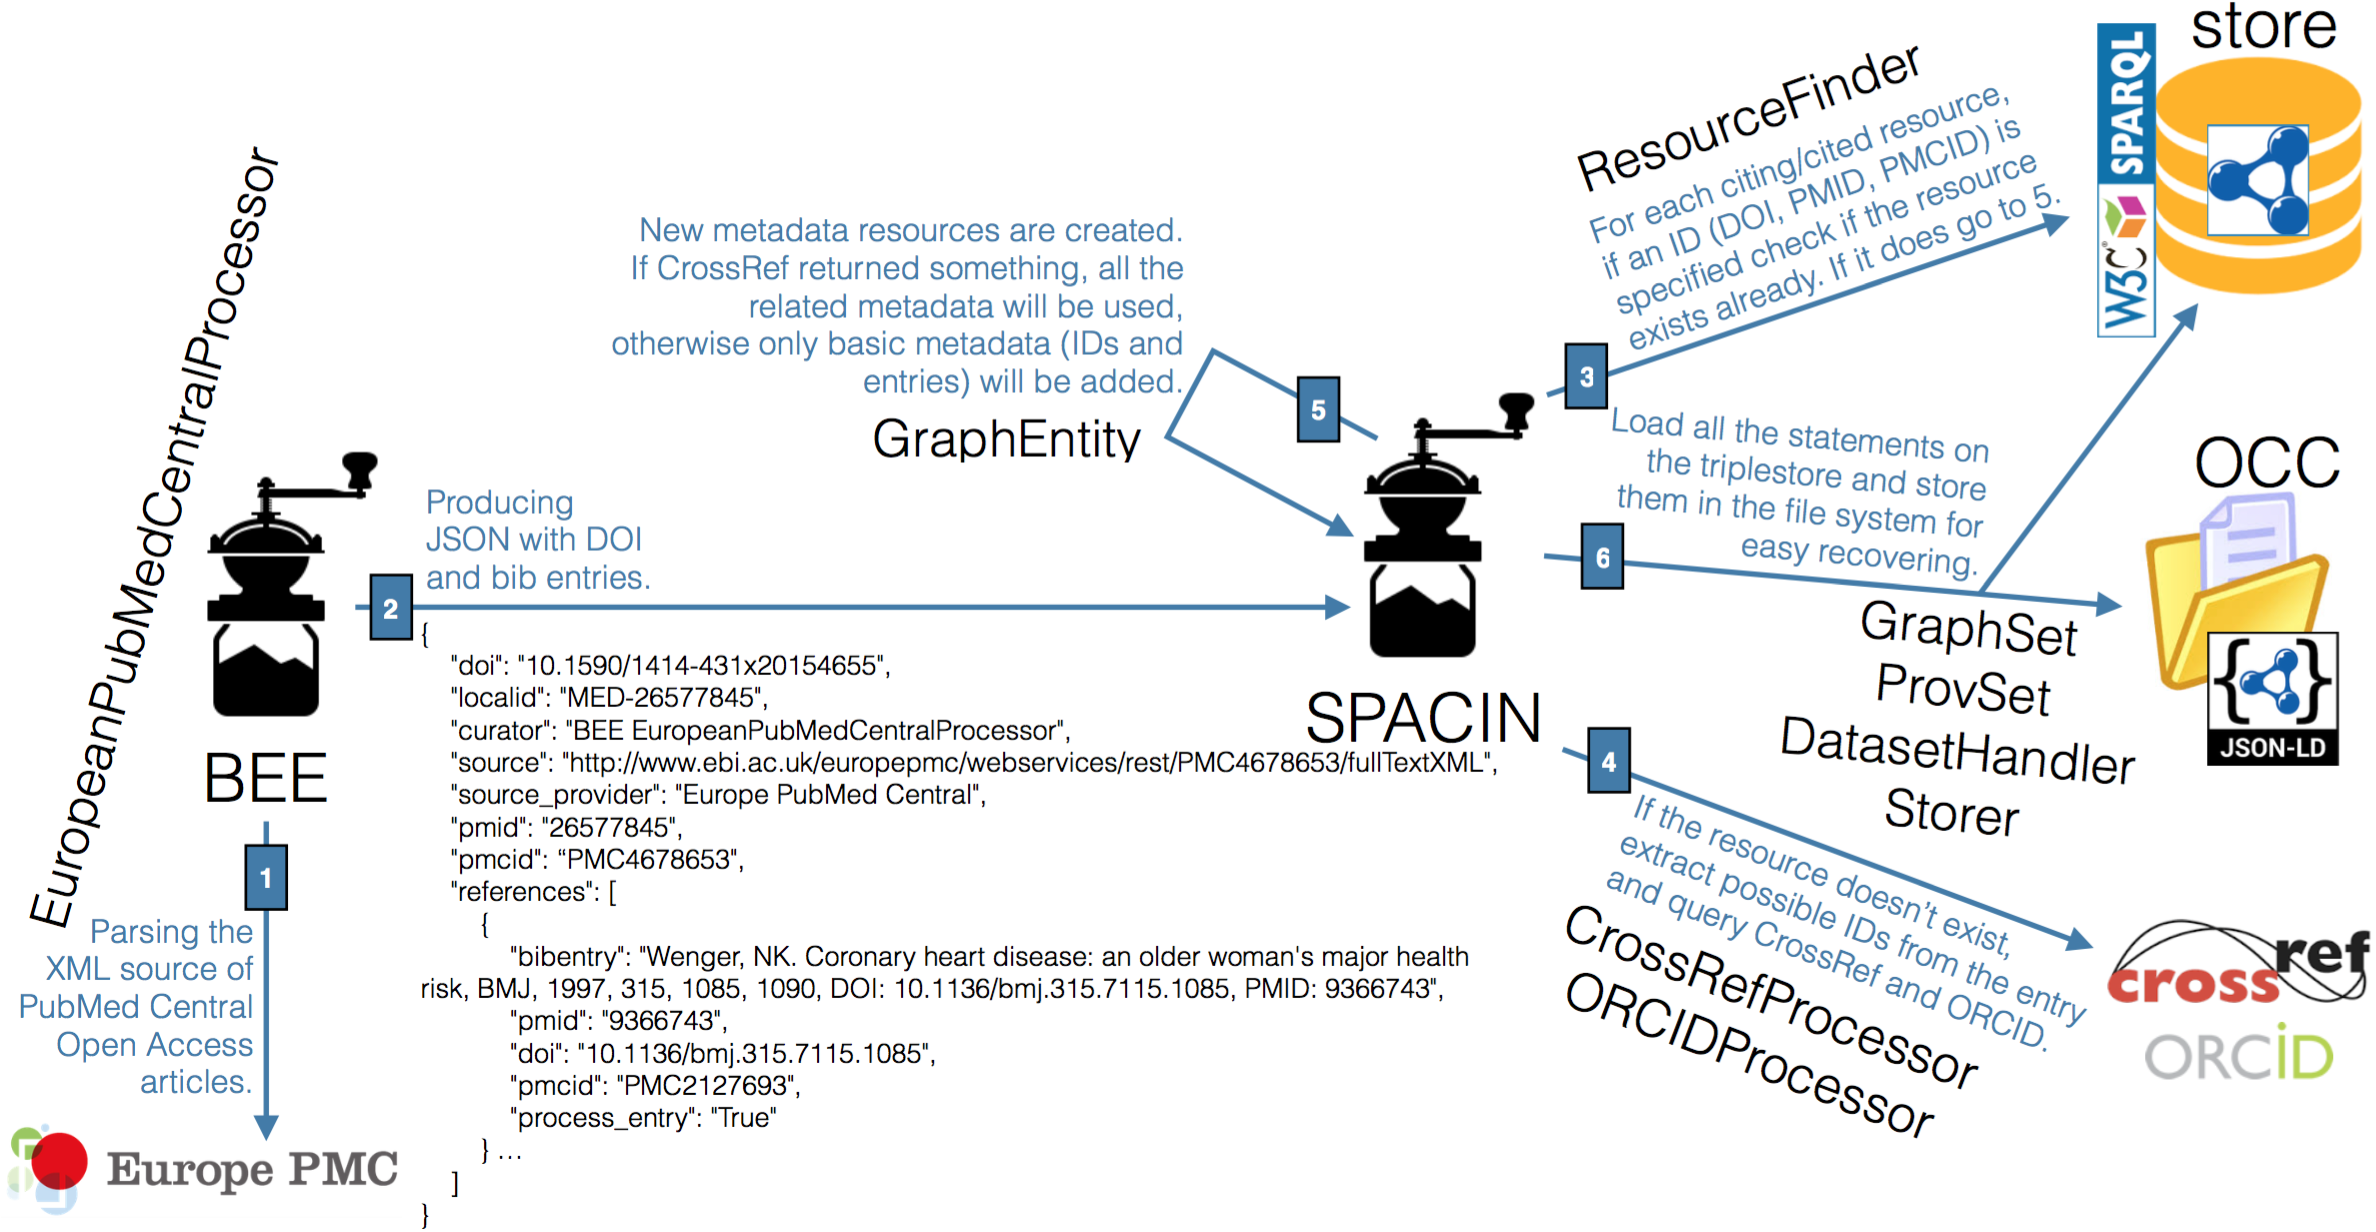
\includegraphics[width=\maxwidth{\textwidth}]{img/1000020100000948000004D0192123CB.png}
\cprotect\caption{The steps involving BEE and SPACIN, and their related Python classes, in the production of the OpenCitations Corpus.}
\label{refIllustration0}
\end{figure}


We have tested the performances of SPACIN in processing the JSON files generated by BEE and produce new RDF resources for the OCC. In particular, we run SPACIN on two subsets of JSON file: 67 JSON files describing all 67 papers included in the Proceedings of ISWC 2015, and the first 67 JSON files produced by BEE from the Open Access subset of PubMed Central as the outcome of the experiment described in Section~\ref{__RefHeading__11281_1890349413}. We use the same configuration as before, i.e. a MacBook Pro, with 2 GHz Intel Core i7 processor, 8 GB DDR3 1600 MHz, OS X 10.11.3.

{\bf ISWC 2015 dataset.} SPACIN took 45 minutes to process all 67 papers in the ISWC 2015 Proceedings, and the outcomes have been published in  \cite{__RefNumPara__5447_1890349413}. Each citing paper contained about 23 references on average, and SPACIN produced 1,441 new citing/cited resources, for a total of 1,531 citation links. These resources are contained in 411 different container resources (e.g. journals, proceedings, books), published by 42 distinct publishers. The total number of authors is 3,076, 157 of whom (5.1\%) have been disambiguated through their ORCID. The total number of RDF statements created is 69,995 (which, as explained, excludes provenance data and datasets information), on average 1,044 triples per citing resource.

{\bf Europe PubMed Central dataset.} SPACIN took 210 minutes to process 67 papers from Europe PubMed Central, and the outcomes have been published in  \cite{__RefNumPara__5449_1890349413}. Each citing paper contained about 50 references on average, and SPACIN produced 3391 new citing/cited resources, for a total of 3,337 citation links. These resources are contained in 1,047 different container resources (e.g. journals, proceedings, books), published by 137 distinct publishers. The total number of authors is 21,658, 957 of whom (4.4\%) have been disambiguated through their ORCID identifiers. The total number of RDF statements created is 377,237 (excluding, as before, provenance data and datasets information), on average 5,630 triples per citing resource. This number will reduce as the OCC becomes more fully populated, since more cited resources will already be described within the database.

In Table~\ref{refTable0} we summarise some metrics related to the resources included in the aforementioned exemplar datasets. While these data are far from having a full coverage, they provide interesting snapshots of these two communities. On the one hand, the community of ISWC 2015 is composed by a relatively small number of people. Even if the average number of references per paper is quite small (average 23, the paper with the most references having 47 citation links), there are several papers that were cited more than one time (the most cited one received 7 citations). Many of the citations are to resources for which Crossref was not able to return any metadata. This is understandable, since many citations in these Semantic Web papers are to Web documents (e.g. W3C Recommendations) and to workshop papers not indexed by Crossref (e.g. CEUR Workshop Series\footnote{\url{http://ceur-ws.org/}}). Some of these non-Crossref-indexed publications are well known and well cited within this community (the most cited one has 4 citations within these 67 ISWC papers).
\begin{table}[h!]
\centering

\cprotect\caption{Some aggregated data of the two exemplar datasets produced by SPACIN.}
\renewcommand{\tabularxcolumn}[1]{>{\arraybackslash}m{#1}}
\newcolumntype{Y}{>{\centering\arraybackslash}X}
\newcolumntype{Z}{>{\arraybackslash}X}

\scalebox{0.8} {\begin{tabularx}{1.22\textwidth}{ >{\hsize=0.33333333333333337\hsize}Y  >{\hsize=0.33333333333333337\hsize}Y  >{\hsize=0.33333333333333337\hsize}Y }
\toprule

{\bf Property} & {\bf ISWC 2015} & {\bf Europe PubMed Central} \\
 \toprule

Max. number of bibliographic references within a paper & 47 & 320 \\
 \midrule

Max. number of citations received by a paper within this sample & 7 & 3 \\
 \midrule

Percentage of cited resources for which Crossref did not return any metadata & 44\% & 13\% \\
 \midrule

Max. number of citations received by a cited resource for which Crossref did not return any metadata & 4 & 1 \\
 \bottomrule

\end{tabularx}}

\label{refTable0}
\end{table}


On the other hand, we see a quite different citation behaviour in the Europe PubMed Central papers. In this case, as expected, the number of average references is higher (average 50, with one review paper having 320 citation links). The paper within this small sample that has been cited most received only 3 citations from the other 66 papers, and this is clearly due to the dimension of the citation graph of the Biomedical and Life Science community to which PubMed Central relates, which is clearly bigger and more sparsely linked than the ISWC one. Additionally, these papers usually cite others published in journals to which proper identifiers (e.g. DOIs) have been assigned, explaining the lower percentage of citations to resources that are not indexed by Crossref.

\section{Related works}\label{__RefHeading__5192_1890349413}

In recent years we have seen a growing interest within the Semantic Web community for in creating and making available RDF datasets concerning bibliographic metadata of scholarly documents. While the list of such works is quite extensive, inIn this section we describe four of the most important contributions in the area.

The Semantic Lancet\footnote{\url{http://semanticlancet.eu/}} Project  \cite{__RefNumPara__69_1852566440} aims at building a Linked Open Dataset of scholarly publication metadata starting from the articles published by Elsevier. In particular, the current dataset contains SPAR-based  \cite{__RefNumPara__17_1852566440} metadata about several papers published in the Journal of Web Semantics\footnote{\url{http://www.journals.elsevier.com/journal-of-web-semantics/}}, including citation links marked with the motivations justifying them by means of CiTO properties. It has several graphical interfaces that allow browsing and sense-making of these data.

Springer LOD\footnote{\url{http://lod.springer.com/}} \cite{__RefNumPara__5076_1890349413} is an RDF dataset made available by Springer Nature that publishes Springer metadata about conferences as Linked Open Data (LOD). Its main focus in on proceedings volumes and the related conferences, but it does not contain metadata describing the individual articles contained in such proceedings.

OpenAIRE\footnote{\url{https://www.openaire.eu/}} \cite{__RefNumPara__71_1852566440} is an Horizon 2020 open data project which publishes metadata of more than 14 millions of publications and thousands of datasets. It makes available a mechanism for searching, discovering and monitoring scientific outputs.

Finally, Scholarly Data\footnote{\url{http://www.scholarlydata.org/}} \cite{__RefNumPara__75_1852566440} is a new project that refactors the Semantic Web Dog Food\footnote{\url{http://data.semanticweb.org/}} so as to keep the dataset growing in good health, and that adopts the new Conference Ontology\footnote{\url{https://w3id.org/scholarlydata/ontology/conference-ontology.owl}} (aligned with other existing models including SPAR  \cite{__RefNumPara__17_1852566440}) for describing the data.

\section{Conclusions}\label{__RefHeading__171_1852566440}

In this paper we have introduced the OpenCitations Project, which has created an open repository of accurate bibliographic references harvested from the scholarly literature: the OpenCitations Corpus (OCC). The new instance of the OCC has recently been established, and is already populated with data describing 595,222 citation links (as of August 24, 2016) -- a number that will grow quickly over the coming months as the continuous workflow adds new data dynamically from Europe PubMed Central and other authoritative sources. The OCC SPARQL endpoint is presently available for use, and distributions of the OCC datasets will shortly be made openly available for bulk download -- the first of these by early September 2016, with subsequent incremental additions.

We are currently working on two different aspects. First of all, we are developing tools for linking the resources within the OCC with those included in other datasets, e.g. Scholarly Data and Springer LOD. In addition, we are experimenting with the use of multiple parallel instantiations of SPACIN, so as to increase the amount of new information that can be processed daily into OCC. 

\subsubsection*{Acknowledgements.}All the scripts used in OpenCitations have been developed as outcomes of several personal communications with people responsible for the external services that OCC uses. We would like to thank leading people in Europe PubMed Central (in particular Johanna McEntyre and Vid Vartak), Crossref (in particular Ed Pentz, Geoffrey Bilder, and Karl Ward) and ORCID (in particular Josh Brown and Laurel Hack) for their help. We would also like to thank Alfred Hofmann and Aliaksandr Birukou (Springer Nature) for allowing us to publish in Figshare the OCC metadata concerning the Proceedings of ISWC 2015  \cite{__RefNumPara__5447_1890349413}, which they kindly provided us in XML.


\begin{thebibliography}{4}

\bibitem{__RefNumPara__71_1852566440} Alexiou, G., Vahdati, S., Lange, C., Papastefanatos G., Lohmann, S. (2016). OpenAIRE LOD services: Scholarly Communication Data as Linked Data. To appear in Proceedings of SAVE-SD 2016. \url{http://cs.unibo.it/save-sd/2016/papers/html/alexiou-savesd2016.html}
\bibitem{__RefNumPara__69_1852566440} Bagnacani, A., Ciancarini, P., Di Iorio, A., Nuzzolese, A. G., Peroni, S., Vitali, F. (2014). The Semantic Lancet Project: A Linked Open Dataset for Scholarly Publishing. In EKAW 2014 Satellite Events: 101--105. \url{http://dx.doi.org/10.1007/978-3-319-17966-7\_10}
\bibitem{__RefNumPara__5076_1890349413} Bryl, V., Birukou, A., Eckert, K., Kessler, M. (2014). What's in the proceedings? Combining publisher's and researcher's perspectives. In Proceedings of SePublica 2014. \url{http://ceur-ws.org/Vol-1155/paper-01.pdf}
\bibitem{__RefNumPara__8388_1890349413} Di Iorio, A., Nuzzolese, A. G., Peroni, S., Shotton, D., Vitali, F. (2014). Describing bibliographic references in RDF. In Proceedings of SePublica 2014. \url{http://ceur-ws.org/Vol-1155/paper-05.pdf}
\bibitem{__RefNumPara__6706_524287244} Falco, R., Gangemi, A., Peroni, S., Vitali, F. (2014). Modelling OWL ontologies with Graffoo. In The Semantic Web: ESWC 2014 Satellite Events: 320--325. \url{http://dx.doi.org/10.1007/978-3-319-11955-7\_42}
\bibitem{__RefNumPara__75_1852566440} Nuzzolese, A. G., Gentile, A. L., Presutti, V., Gangemi, A. (2016). Conference Linked Data -- Our Web Dog Food has gone gourmet. To appear in Proceedings of ISWC 2016.
\bibitem{__RefNumPara__17_1852566440} Peroni, S. (2014). The Semantic Publishing and Referencing Ontologies. In Semantic Web Technologies and Legal Scholarly Publishing: 121--193. \url{http://dx.doi.org/10.1007/978-3-319-04777-5\_5}
\bibitem{__RefNumPara__293_1852566440} Peroni, S., Dutton, A., Gray, T., Shotton, D. (2015). Setting our bibliographic references free: towards open citation data. Journal of Documentation, 71 (2): 253--277. \url{http://dx.doi.org/10.1108/JD-12-2013-0166}
\bibitem{__RefNumPara__7775_1890349413} Peroni, S., Shotton, D. (2012). FaBiO and CiTO: ontologies for describing bibliographic resources and citations. In Journal of Web Semantics, 17: 33-43. \url{http://dx.doi.org/10.1016/j.websem.2012.08.001}
\bibitem{__RefNumPara__5449_1890349413} Peroni, S., Shotton, D. (2016). Exemplar OCC dataset from Europe PubMed Central metadata. Figshare. \url{https://dx.doi.org/10.6084/m9.figshare.3481922}
\bibitem{__RefNumPara__5447_1890349413} Peroni, S., Shotton, D. (2016). Exemplar OCC dataset from Springer Nature metadata. Figshare. \url{https://dx.doi.org/10.6084/m9.figshare.3481949}
\bibitem{__RefNumPara__19_1852566440} Peroni, S., Shotton, D. (2016). Metadata for the OpenCitations Corpus. Figshare. \url{https://dx.doi.org/10.6084/m9.figshare.3443876}
\bibitem{__RefNumPara__7993_1890349413} Peroni, S., Shotton, D., Vitali, F. (2012). Scholarly publishing and the Linked Data: describing roles, statuses, temporal and contextual extents. In Proceedings of i-Semantics 2012: 9--16. \url{http://dx.doi.org/10.1145/2362499.2362502}
\bibitem{__RefNumPara__6041_1890349413} Shotton, D. (2013). Open Citations. Nature, 502 (7471): 295--297. \url{http://dx.doi.org/10.1038/502295a}

\end{thebibliography}

\end{document}